\documentclass[journal,12pt,twocolumn]{IEEEtran}

\usepackage{setspace}
\usepackage{gensymb}
\singlespacing
\usepackage[cmex10]{amsmath}
\usepackage{amssymb}
\usepackage{xurl}
\usepackage{tabularx}
\usepackage{amsthm}
\usepackage{comment}
\usepackage{mathrsfs}
\usepackage{txfonts}
\usepackage{stfloats}
\usepackage{bm}
\usepackage{cite}
\usepackage{cases}
\usepackage{subfig}
\usepackage{amsmath}
\usepackage{longtable}
\usepackage{multirow}
\usepackage{multicol}

\usepackage{enumitem}
\usepackage{mathtools}
\usepackage{steinmetz}
\usepackage{tikz}
\usepackage{circuitikz}
\usepackage{verbatim}
\usepackage{tfrupee}
\usepackage[breaklinks=true]{hyperref}
\usepackage{graphicx}
\usepackage{tkz-euclide}

\usetikzlibrary{calc,math}
\usepackage{listings}
    \usepackage{color}                                            %%
    \usepackage{array}                                            %%
    \usepackage{longtable}                                        %%
    \usepackage{calc}                                             %%
    \usepackage{multirow}                                         %%
    \usepackage{hhline}                                           %%
    \usepackage{ifthen}                                           %%
    \usepackage{lscape}     
\usepackage{multicol}
\usepackage{chngcntr}

\DeclareMathOperator*{\Res}{Res}

\renewcommand\thesection{\arabic{section}}
\renewcommand\thesubsection{\thesection.\arabic{subsection}}
\renewcommand\thesubsubsection{\thesubsection.\arabic{subsubsection}}

\renewcommand\thesectiondis{\arabic{section}}
\renewcommand\thesubsectiondis{\thesectiondis.\arabic{subsection}}
\renewcommand\thesubsubsectiondis{\thesubsectiondis.\arabic{subsubsection}}


\hyphenation{op-tical net-works semi-conduc-tor}
\def\inputGnumericTable{}                                 %%

\lstset{
%language=C,
frame=single, 
breaklines=true,
columns=fullflexible
}
\begin{document}


\newtheorem{theorem}{Theorem}[section]
\newtheorem{problem}{Problem}
\newtheorem{proposition}{Proposition}[section]
\newtheorem{lemma}{Lemma}[section]
\newtheorem{corollary}[theorem]{Corollary}
\newtheorem{example}{Example}[section]
\newtheorem{definition}[problem]{Definition}

\newcommand{\BEQA}{\begin{eqnarray}}
\newcommand{\EEQA}{\end{eqnarray}}
\newcommand{\define}{\stackrel{\triangle}{=}}
\bibliographystyle{IEEEtran}
\raggedbottom
\setlength{\parindent}{0pt}
\providecommand{\mbf}{\mathbf}
\providecommand{\pr}[1]{\ensuremath{\Pr\left(#1\right)}}
\providecommand{\qfunc}[1]{\ensuremath{Q\left(#1\right)}}
\providecommand{\sbrak}[1]{\ensuremath{{}\left[#1\right]}}
\providecommand{\lsbrak}[1]{\ensuremath{{}\left[#1\right.}}
\providecommand{\rsbrak}[1]{\ensuremath{{}\left.#1\right]}}
\providecommand{\brak}[1]{\ensuremath{\left(#1\right)}}
\providecommand{\lbrak}[1]{\ensuremath{\left(#1\right.}}
\providecommand{\rbrak}[1]{\ensuremath{\left.#1\right)}}
\providecommand{\cbrak}[1]{\ensuremath{\left\{#1\right\}}}
\providecommand{\lcbrak}[1]{\ensuremath{\left\{#1\right.}}
\providecommand{\rcbrak}[1]{\ensuremath{\left.#1\right\}}}
\theoremstyle{remark}
\newtheorem{rem}{Remark}
\newcommand{\sgn}{\mathop{\mathrm{sgn}}}
\providecommand{\abs}[1]{\vert#1\vert}
\providecommand{\res}[1]{\Res\displaylimits_{#1}} 
\providecommand{\norm}[1]{\lVert#1\rVert}
%\providecommand{\norm}[1]{\lVert#1\rVert}
\providecommand{\mtx}[1]{\mathbf{#1}}
\providecommand{\mean}[1]{E[ #1 ]}
\providecommand{\fourier}{\overset{\mathcal{F}}{ \rightleftharpoons}}
%\providecommand{\hilbert}{\overset{\mathcal{H}}{ \rightleftharpoons}}
\providecommand{\system}{\overset{\mathcal{H}}{ \longleftrightarrow}}
	%\newcommand{\solution}[2]{\textbf{Solution:}{#1}}
\newcommand{\solution}{\noindent \textbf{Solution: }}
\newcommand{\cosec}{\,\text{cosec}\,}
\providecommand{\dec}[2]{\ensuremath{\overset{#1}{\underset{#2}{\gtrless}}}}
\newcommand{\myvec}[1]{\ensuremath{\begin{pmatrix}#1\end{pmatrix}}}
\newcommand{\mydet}[1]{\ensuremath{\begin{vmatrix}#1\end{vmatrix}}}
\newcommand*{\permcomb}[4][0mu]{{{}^{#3}\mkern#1#2_{#4}}}
\newcommand*{\perm}[1][-3mu]{\permcomb[#1]{P}}
\newcommand*{\comb}[1][-1mu]{\permcomb[#1]{C}}
\numberwithin{equation}{subsection}
\makeatletter
\@addtoreset{figure}{problem}
\makeatother
\let\StandardTheFigure\thefigure
\let\vec\mathbf
\renewcommand{\thefigure}{\theproblem}
\def\putbox#1#2#3{\makebox[0in][l]{\makebox[#1][l]{}\raisebox{\baselineskip}[0in][0in]{\raisebox{#2}[0in][0in]{#3}}}}
     \def\rightbox#1{\makebox[0in][r]{#1}}
     \def\centbox#1{\makebox[0in]{#1}}
     \def\topbox#1{\raisebox{-\baselineskip}[0in][0in]{#1}}
     \def\midbox#1{\raisebox{-0.5\baselineskip}[0in][0in]{#1}}
\vspace{3cm}
\title{Assignment 3}
\author{CS20BTECH11047}
\maketitle
\newpage
\bigskip
\renewcommand{\thefigure}{\arabic{figure}}
\renewcommand{\thetable}{\arabic{table}}
Download all python codes from 
\begin{lstlisting}
https://github.com/JeevanIITH/AI1102/blob/main/
assignment3/assignment3.py
\end{lstlisting}
%
and latex codes from 
%
\begin{lstlisting}
https://github.com/JeevanIITH/AI1102/blob/main/
assignment3/assignment3.tex
\end{lstlisting}
\section*{GATE EC 2012 Q.1}
Two independent random variables $X$ and $Y$ are uniformly distributed in the interval [-1,1]. The probability that $\max \brak{X,Y}$ is less than $\dfrac{1}{2}$ is 
\begin{multicols}{4}
\begin{enumerate}
\item $\dfrac{3}{4}$
\item $\dfrac{9}{16}$
\item $\dfrac{1}{4}$
\item $\dfrac{2}{3}$
\end{enumerate}
\end{multicols}

\section*{Solution}
 Since the random variable $X$ is uniformly distributed in the interval [-1,1],let $f_{X}(x)=k$.Then
 \begin{align}
 \int_{-1}^{1}f_{X}(x) dx = \int_{-1}^{1} k dx=1\\
 \Rightarrow k=\dfrac{1}{2} \\
 \intertext{So}  f_{X}(x) = \dfrac{1}{2}  \quad ,  x \in (-1,1)\\
 \intertext{Similarly}  f_{Y}(y) = \dfrac{1}{2}  \quad ,  y \in (-1,1)
 \end{align}
Now
 \begin{align}
 \max\brak{X,Y} < \dfrac{1}{2} \Rightarrow  \left(X<\dfrac{1}{2}\right) . \left(Y<\dfrac{1}{2}\right)\\
 \intertext{So} \pr{\max \brak{X,Y} < \dfrac{1}{2}}= \pr{\left(X<\dfrac{1}{2}\right) . \left(Y<\dfrac{1}{2}\right)  }
 \end{align}
 Since $X$ and $Y$ are independent 
 \begin{align}
 \label{eq:7}
 \pr{\left(X<\dfrac{1}{2}\right) . \left(Y<\dfrac{1}{2}\right)  } = \pr{ X<\dfrac{1}{2} } \times  \pr{Y<\dfrac{1}{2} }
 \end{align}
 Now using CDF
 \begin{align}
 F_{X}(x)=\pr{ X<x }= \int _{-1}^{x} f_{X}(x) dx\\
 = \int _{-1}^{x} \dfrac{1}{2} dx= \dfrac{1}{2} \left( x-(-1) \right) = \dfrac{1}{2}( x+1) 
 \intertext{so} F_{X}(x)=\begin{cases}
 0   &   x<-1\\
 \dfrac{1}{2} (x+1) &   -1<x<1\\
 1  &   x>1 
 \end{cases}
  \label{eq:9}
 \intertext{similarly} F_{Y}(y)= \pr{Y<y } = \int _{-1}^{y} f_{Y}(y) dy\\
 = \int _{-1}^{y} \dfrac{1}{2} dy= \dfrac{1}{2} \left( y-(-1) \right) =\dfrac{1}{2}(y+1)
 \intertext{so} F_{Y}(y)=\begin{cases}
 0 & y<-1\\
 \dfrac{1}{2} (y+1)  &  -1<y<1\\
 1  & y>1 
 \end{cases} 
 \label{eq:11}
 \end{align}
Using  \eqref{eq:9} and \eqref{eq:11} in \eqref{eq:7} we get
\begin{align}
\pr{\max\brak{X,Y} < \dfrac{1}{2}}=F_{X}\left(\dfrac{1}{2} \right)\times F_{Y}\left(\dfrac{1}{2} \right)\\
=\dfrac{1}{2} \left(\dfrac{1}{2}+ 1 \right) \times \dfrac{1}{2} \left( \dfrac{1}{2}+1 \right)=\dfrac{3}{4} \times \dfrac{3}{4}= \dfrac{9}{16}
\end{align} 
So option 2 is correct answer 
\begin{figure}[h]
    \centering
    %\columnwidth
    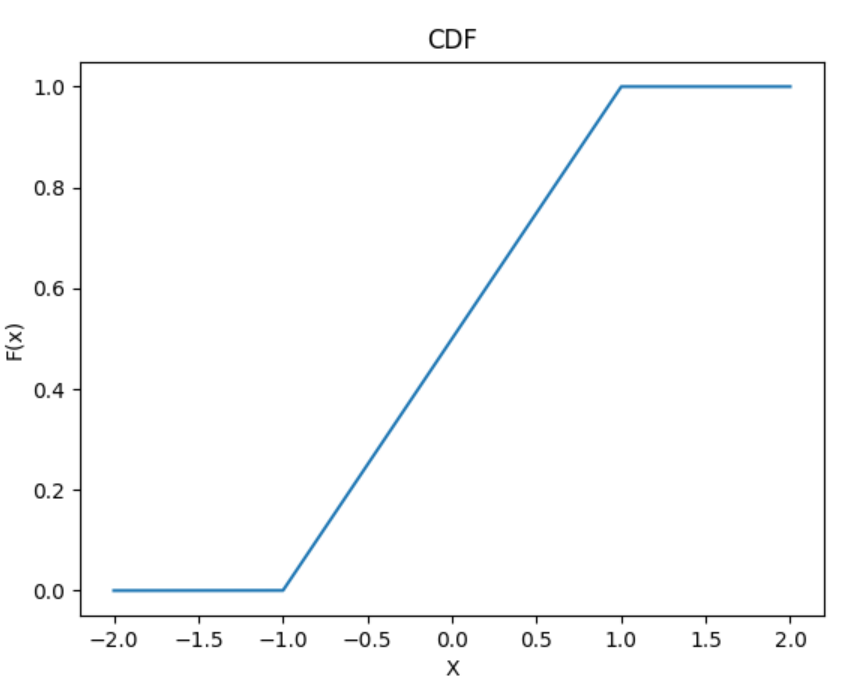
\includegraphics[width=\columnwidth]{cdf.png}
    \caption{$F_{X}(x)$}
    \label{fig:$F_{X}(x)$}
\end{figure}














\end{document}
